
\chapter{Imagens} \label{imagens}

A utilização de imagens em trabalhos acadêmicos é muito comum, de 
modo que a manipulação de imagens merece uma atenção especial. 
Todos os mecanismo do \LaTeX\ para a manipulação de imagens podem 
ser utilizados com a classe \estilo, mas algumas tarefas mais 
rotineiras podem ter sua execução otimizada.

Embora a classe estilo possa ser utilizada com qualquer tipo de 
imagem, a configuração padrão aceita apenas os formatos mais 
comuns, a saber: .jpg, .png e .pdf. Adotar esses formatos como 
padrão justifica-se por que eles são extremamente comuns. O 
conteúdo desse capítulo presume que o arquivo da imagem esteja em 
um desses formatos.


\section{Inclusão de imagem}


Imagens são diferentes dos outros elementos que compõem um texto, em
nenhuma circunstância podem ser divididas e devem vir acompanhadas 
de legenda e/ou referência.

Para inserir imagem usa-se o comando \cmc{includegraphics}{arquivo}, 
são aceitas imagens nos formatos .jpg, .png, .pdf quando o objetivo 
é gerar pdf direto do tex, se for gerar dvi sua imagem precisa 
estar no formato .ps ou .eps.
\begin{tcolorbox}
\begin{lstlisting}
    
\includegraphics{Logo} %%% insere a imagem
\end{lstlisting}
\end{tcolorbox}

\includegraphics{Logo}

A classe estilo procura as imagens primeiro em uma pasta 
chamada "\textsf{Imagens}"\, que deve estar no mesmo 
diretório de seu arquivo tex, se essa pasta não existir 
a imagem será procurada na mesma pasta do arquivo tex, 
se o arquivo não existir a compilação falhará e será 
exibida a mensagem de erro:
\textit{File (nome do arquivo) not found}.

O comando \cmc{includegraphics}{arquivo} apenas insere 
a imagem, para que tenha legenda é necessário colocá-la 
dentro de um ambiente \verb|figure|, onde também é 
possível controlar seu posicionamento horizontal.
\begin{tcolorbox}
\begin{lstlisting}
\begin{figure}[H]
    \centering %%% Centraliza a imagem
    
\includegraphics{Logo} %%% Insere a imagem
    \caption{Este é o logotipo da UFRRJ} %%% Legenda da imagem
    \label{Logorural} %%% Marca para fazer referência cruzada
\end{figure}
\end{lstlisting}
\end{tcolorbox}
\begin{figure}[H]
	\centering %%% centraliza a imagem
	
\includegraphics{Logo}
	\caption{Este é o logotipo da UFRRJ} %%% legenda da imagem
	\label{Logorural} %%% Marca para fazer referência cruzada
\end{figure}

O controle do tamanho da imagem é feito pela chave \epar{scale}{valor}.

\epar{scale}{0.5}: imagem reduzida à metade de seu tamanho.

\epar{scale}{1} (valor padrão): imagem em tamanho real.

\epar{scale}{1.2}: imagem ampliada em $20\%$.

\epar{scale}{2}: imagem ampliada em $100\%$, ou seja, dobra de tamanho.

\begin{tcolorbox}
\begin{lstlisting}
\begin{figure}[H]
   \centering
   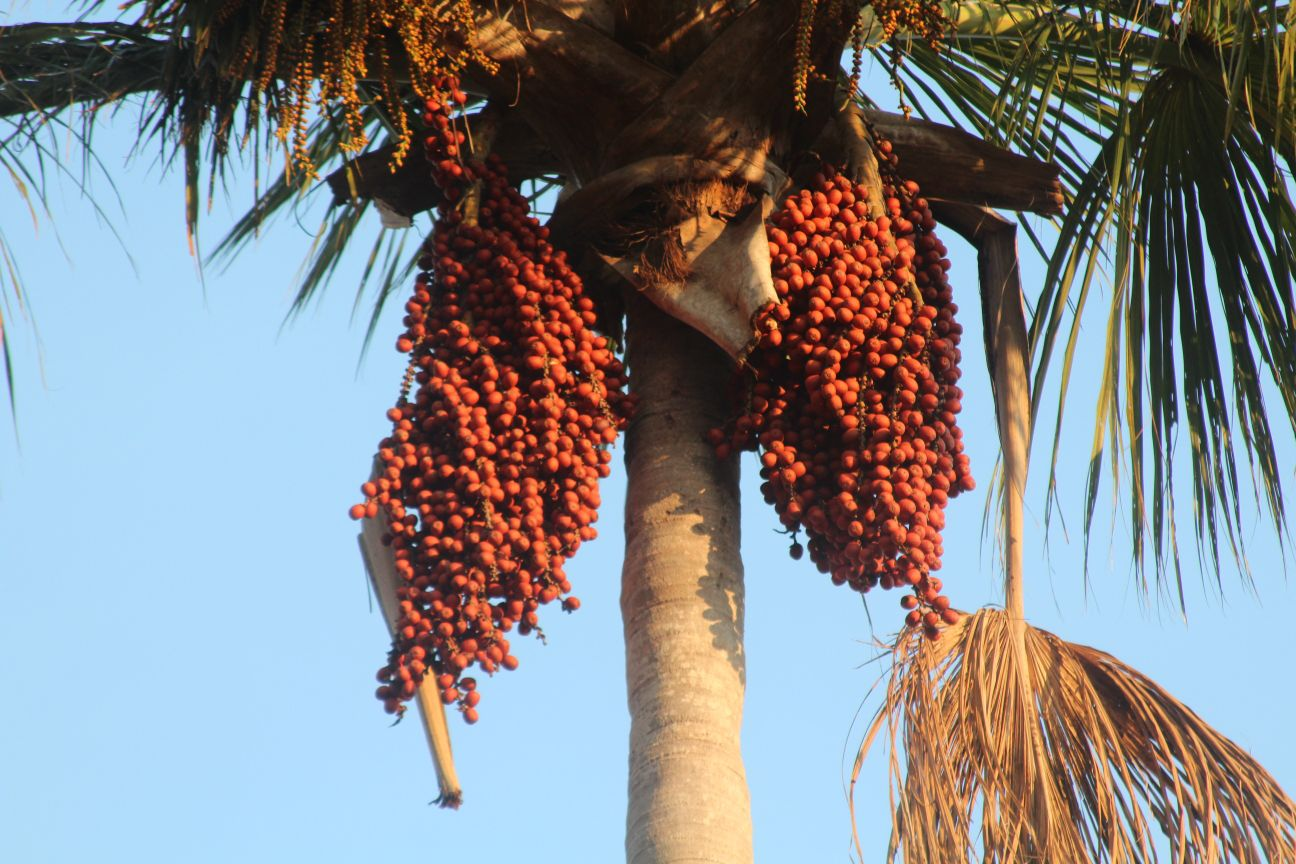
\includegraphics[scale=0.15]{Buriti}
   \caption{Imagem reduzia a $15\%$ do seu tamanho}
\end{figure}
\end{lstlisting}
\end{tcolorbox}

\begin{figure}[H]
   \centering
   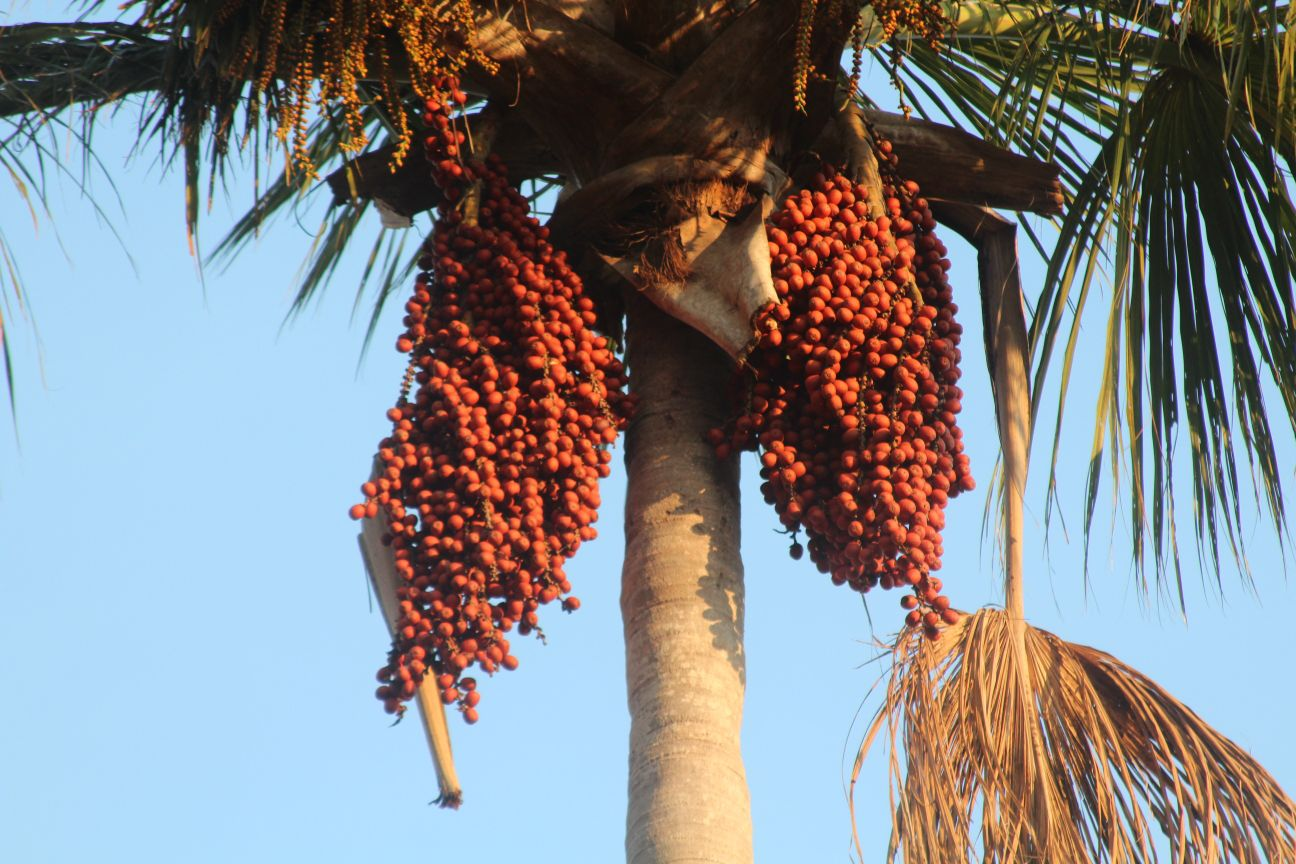
\includegraphics[scale=0.15]{Buriti}
   \caption{Imagem reduzia a $15\%$ do seu tamanho}
   \label{primeira}
\end{figure}

Uma opção muito comum ao lidar com imagem consiste em 
ajustar seu tamanho para coincidir com a largura da 
página, o comando \com{resizebox} faz esse ajuste.
\begin{tcolorbox}
\begin{lstlisting}
\begin{figure}[H]
   \resizebox{\textwidth}{!}{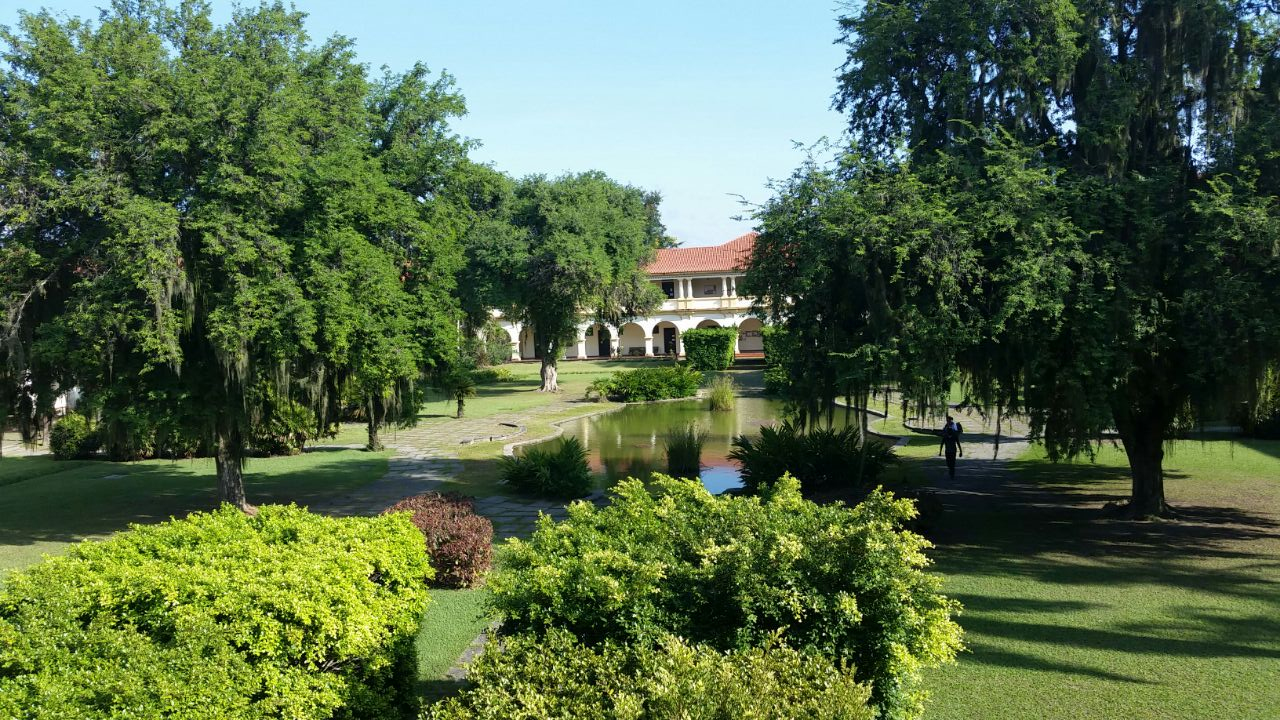
\includegraphics{RuralP1}}
   \caption{O prédio principal da UFRRJ, vulgo P1}
   \label{op1} %%% Marca para referência cruzada
\end{figure}
\end{lstlisting}
\end{tcolorbox}

\begin{figure}[H]
	\resizebox{\textwidth}{!}{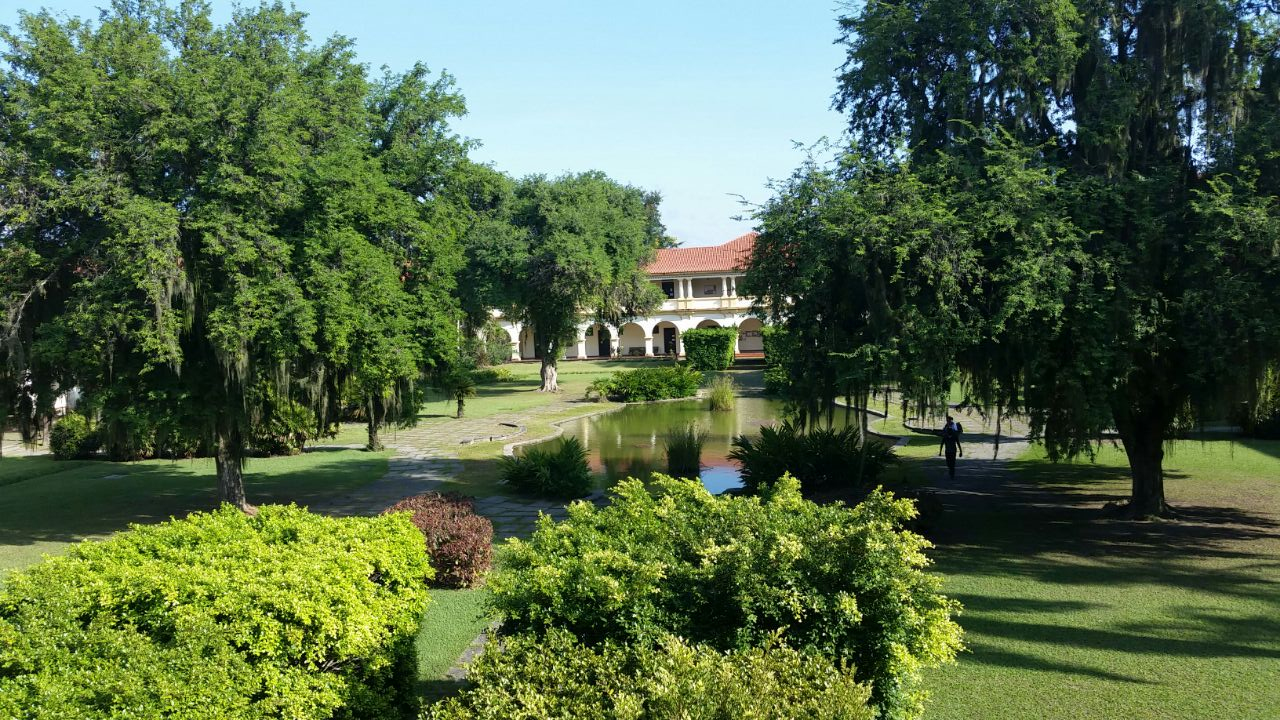
\includegraphics{RuralP1}}
	\caption{O prédio principal da UFRRJ, vulgo P1}
	\label{op1}
\end{figure}

A legenda foi feita com o comando \com{caption}, como esse comando estava abaixo da imagem a legenda ficou abaixo, se esse comando for posto acima da imagem a legenda ficará acima da imagem também. A referência à figura~\ref{op1} foi feita com o comando \cmc{ref}{op1}.

\subsection{Girando de imagem}

É muito simples girar uma imagem no sentido horário ou anti-horário.
\begin{tcolorbox}
\begin{lstlisting}
\begin{figure}[H]
   \centering
   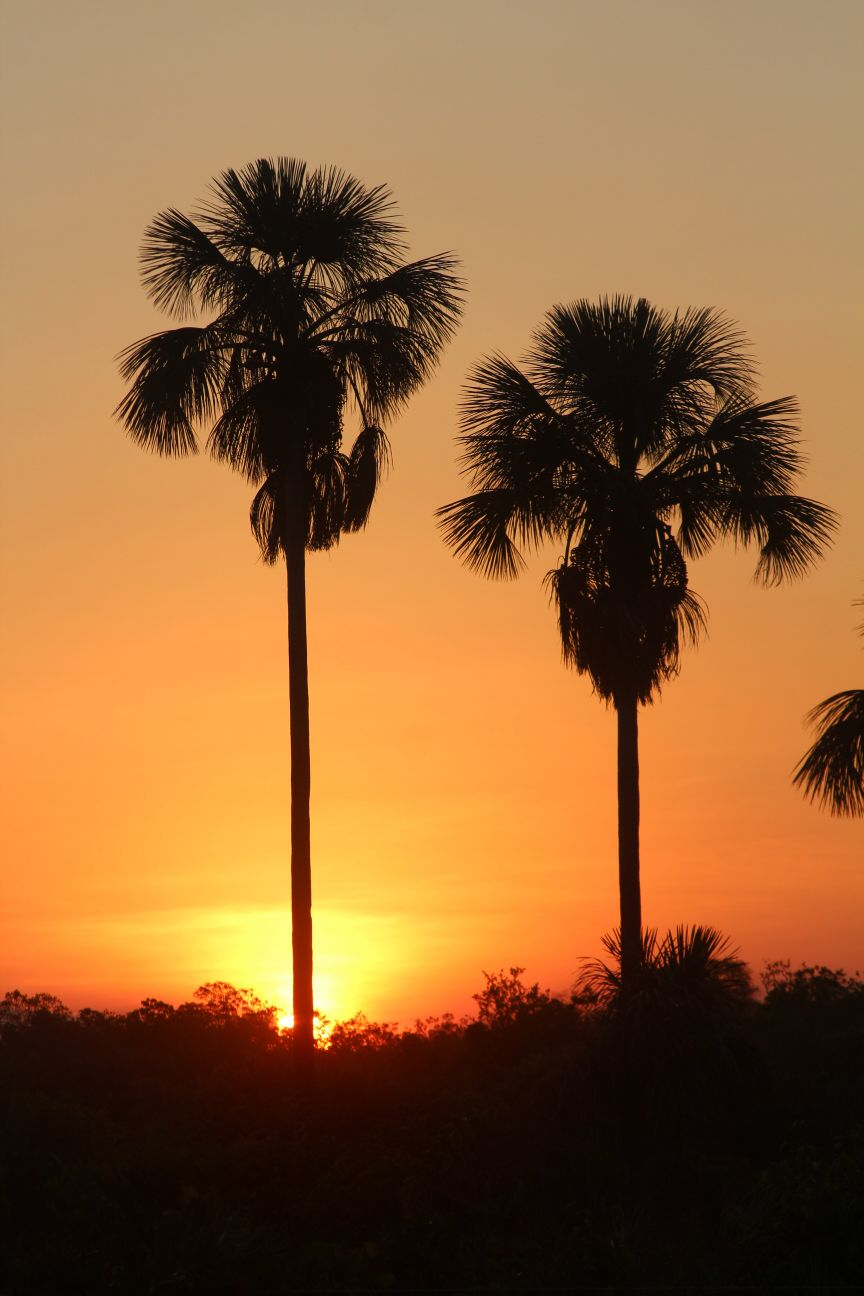
\includegraphics[scale=0.1,angle=-15]{Buritis}
   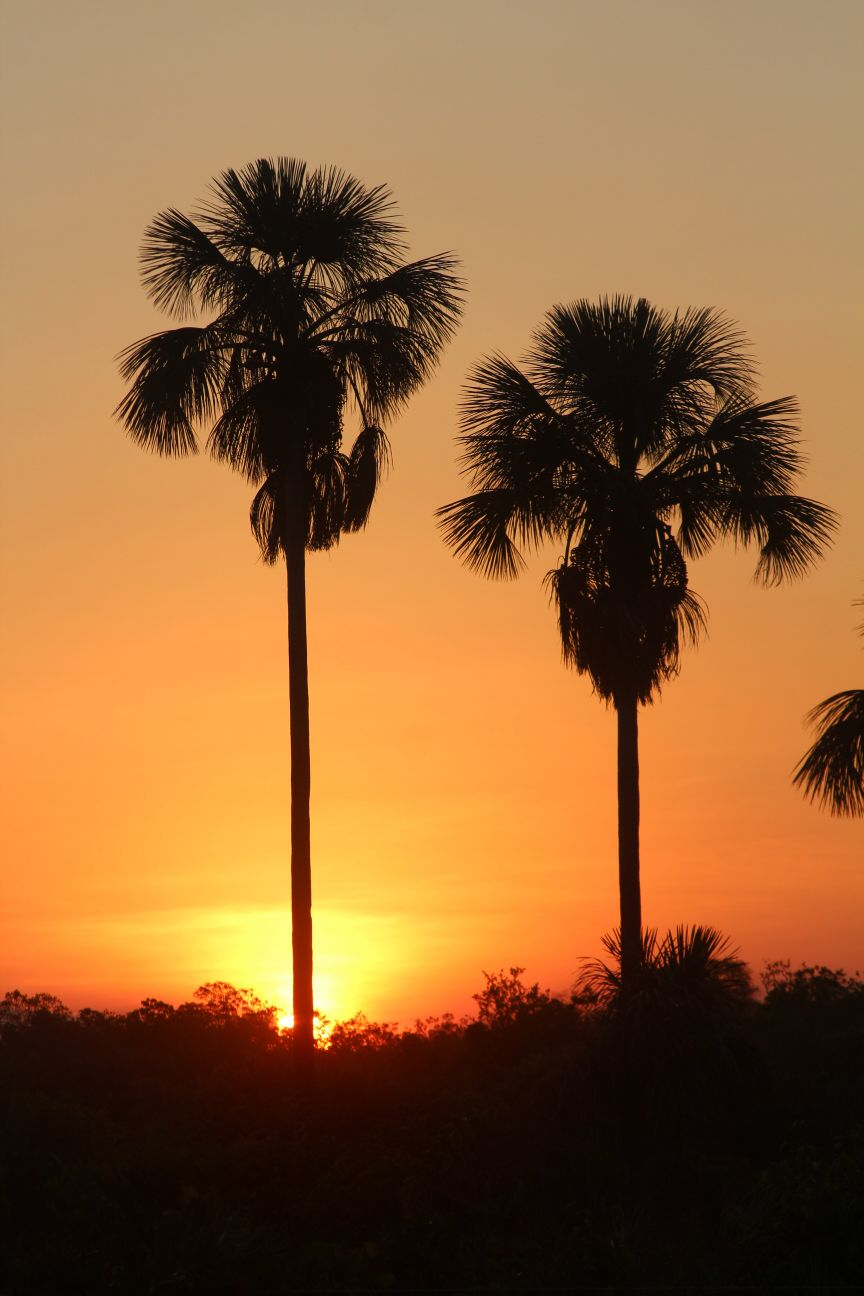
\includegraphics[scale=0.1]{Buritis}
   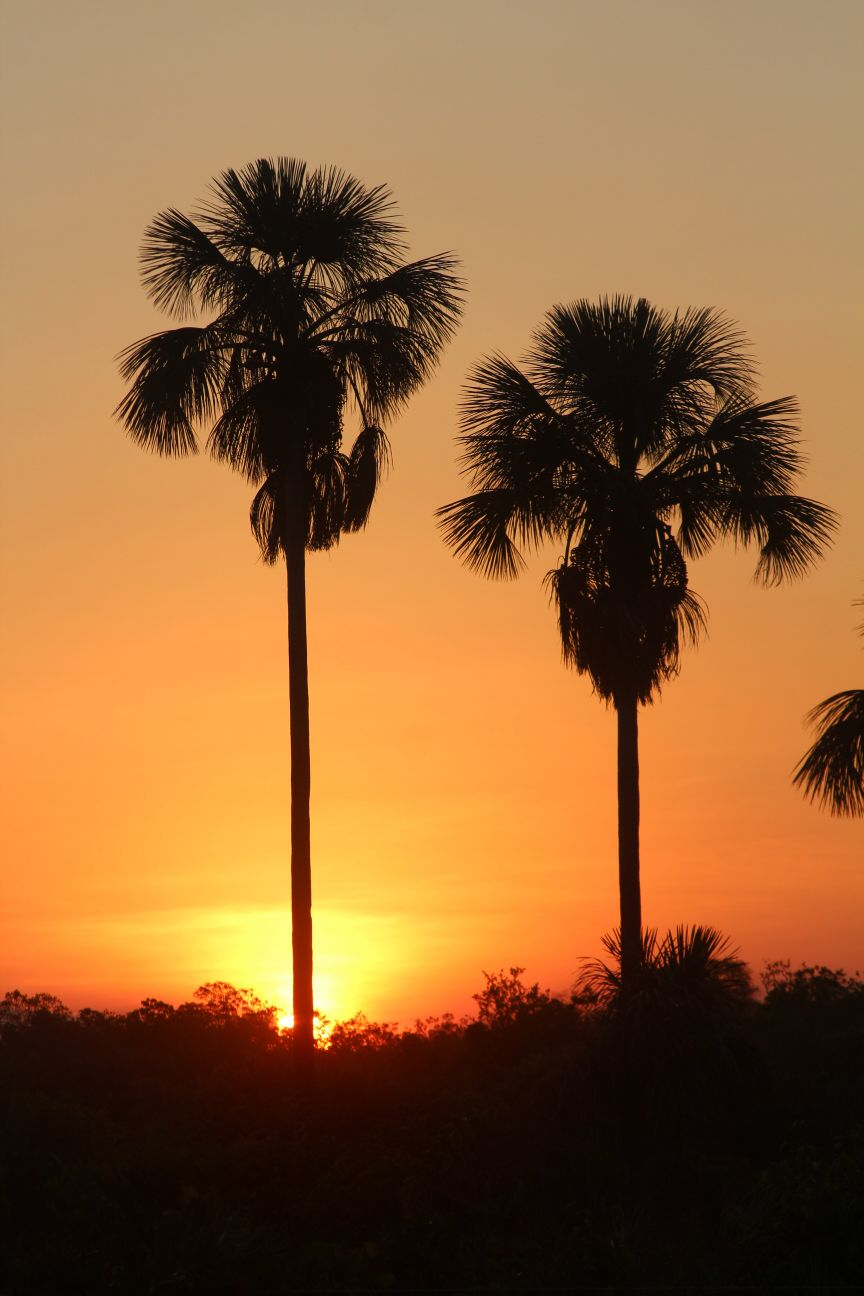
\includegraphics[scale=0.1,angle=15]{Buritis}
   \caption{Girando imagens}\label{giraas}
\end{figure}
\end{lstlisting}
\end{tcolorbox}

\begin{figure}[H]
	\centering
	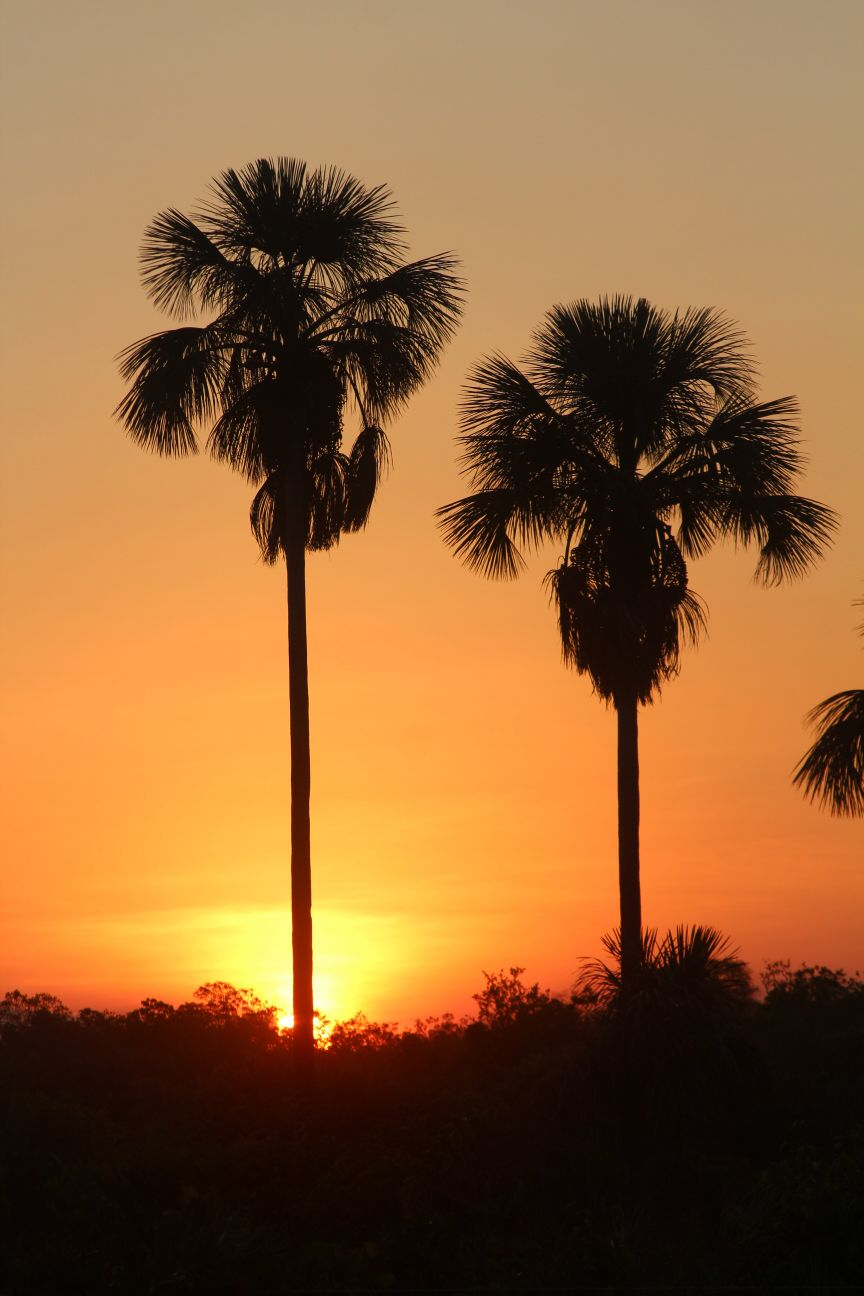
\includegraphics[scale=0.1,angle=-15]{Buritis}
	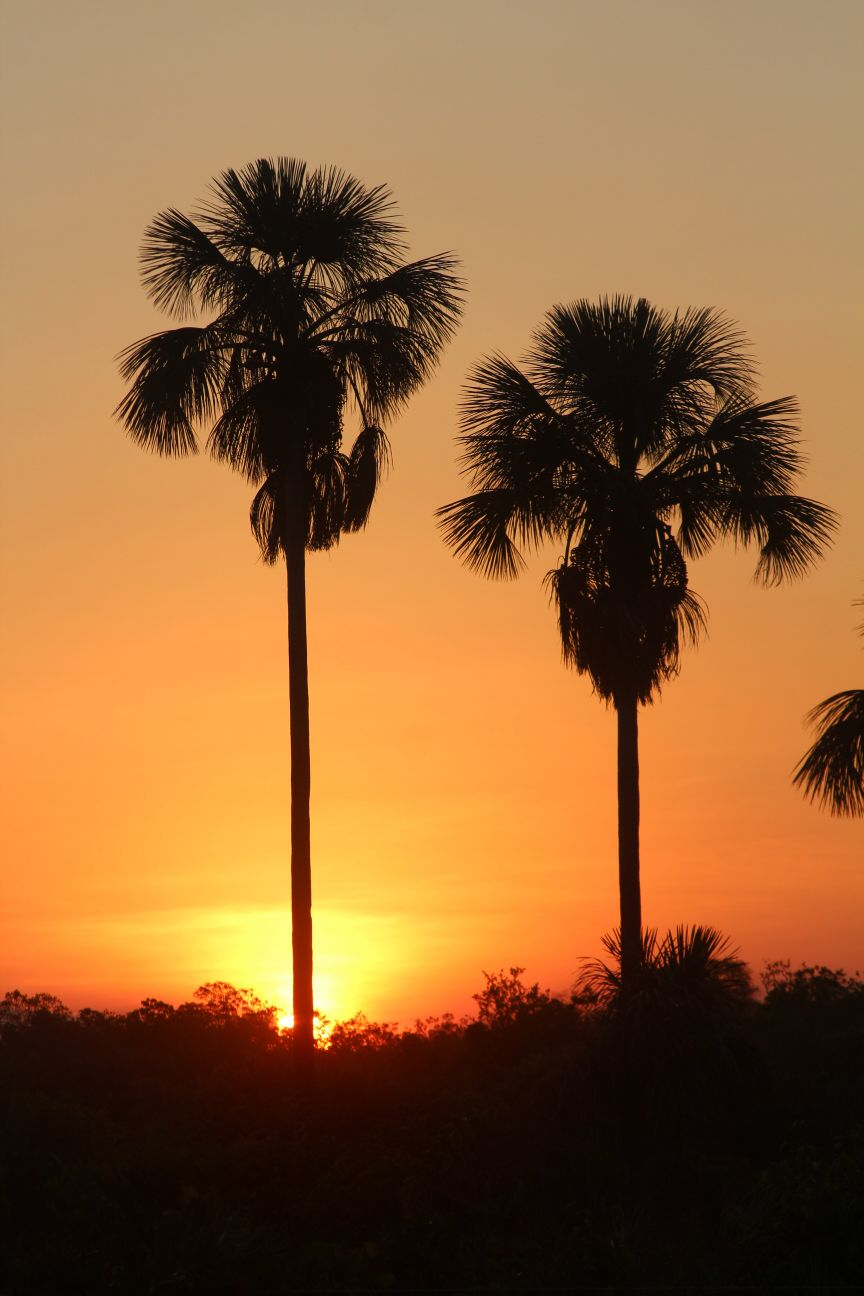
\includegraphics[scale=0.1]{Buritis}
	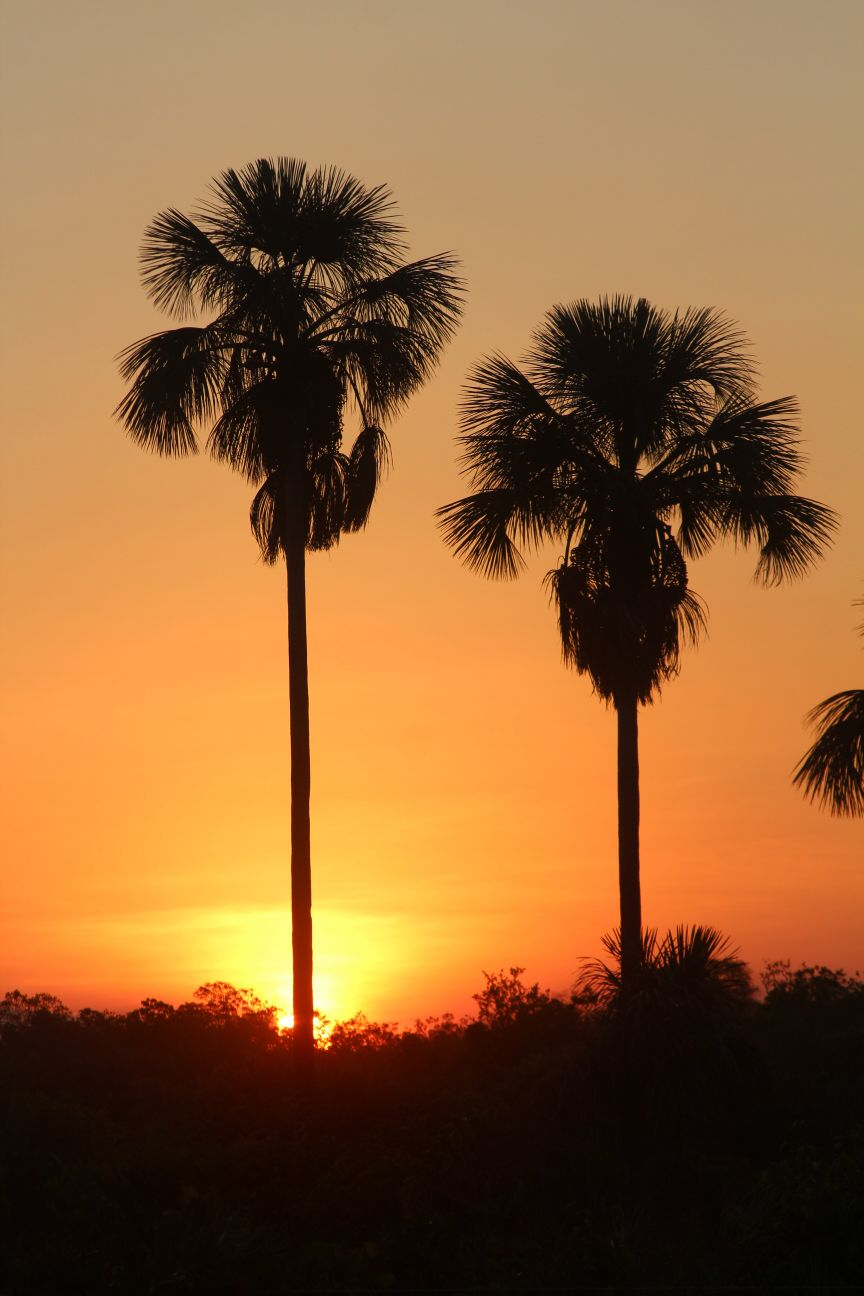
\includegraphics[scale=0.1,angle=15]{Buritis}
	\caption{Girando imagens}\label{giraas}
\end{figure}


\subsection{Imagens lado a lado}

\begin{tcolorbox}
\begin{lstlisting}
\begin{figure}[H]
   \centering
   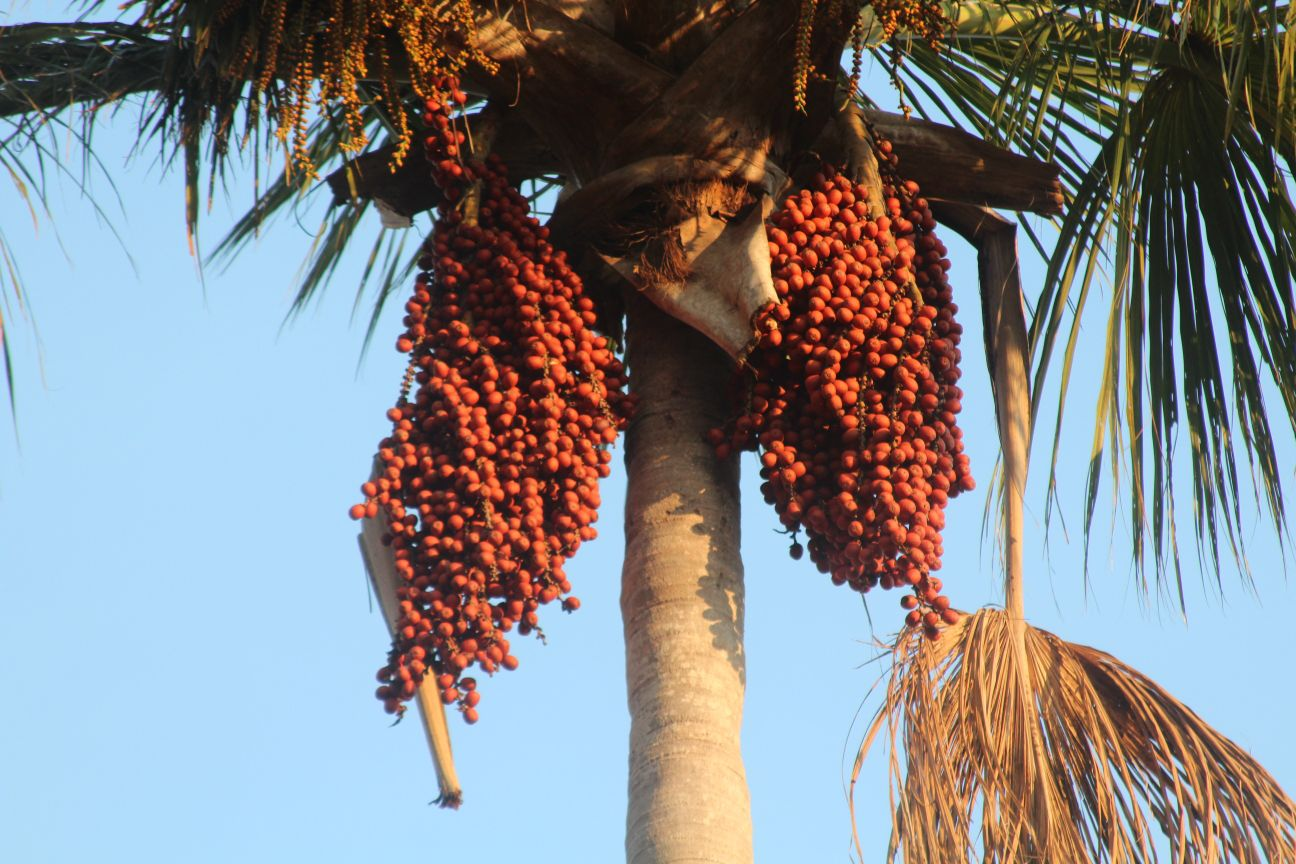
\includegraphics[scale=0.1]{Buriti}
   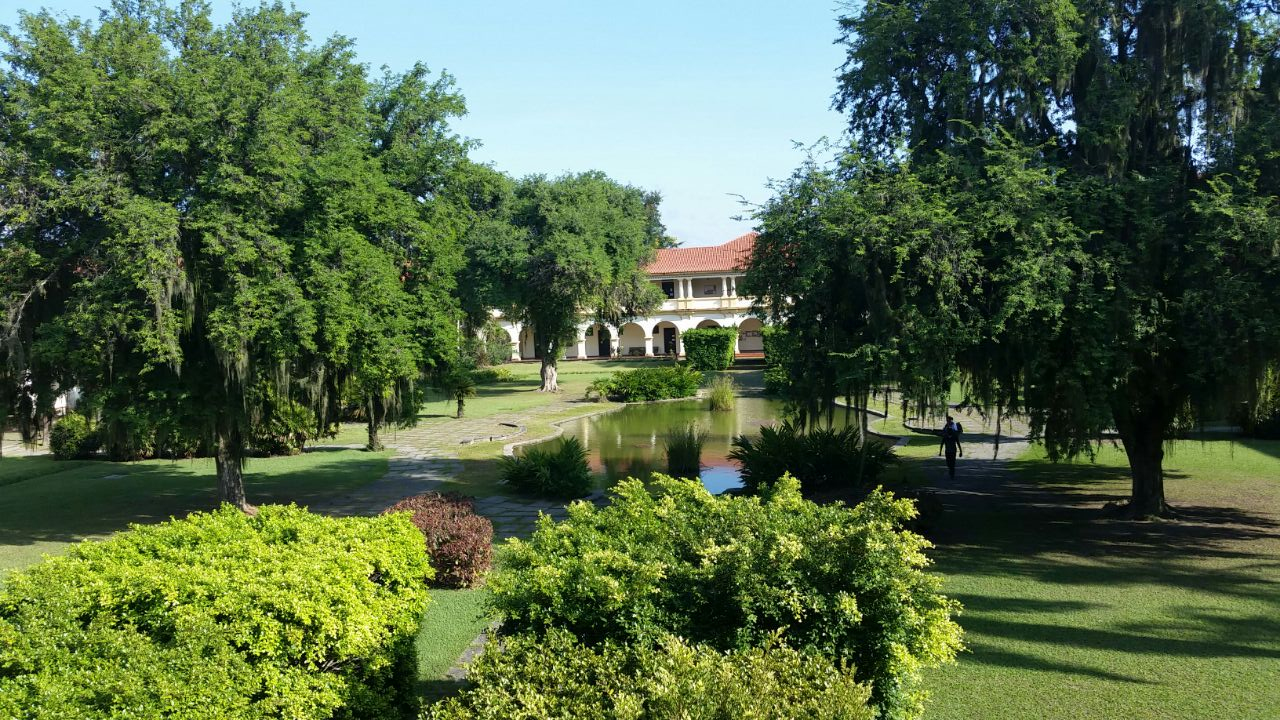
\includegraphics[scale=0.1]{RuralP1}
   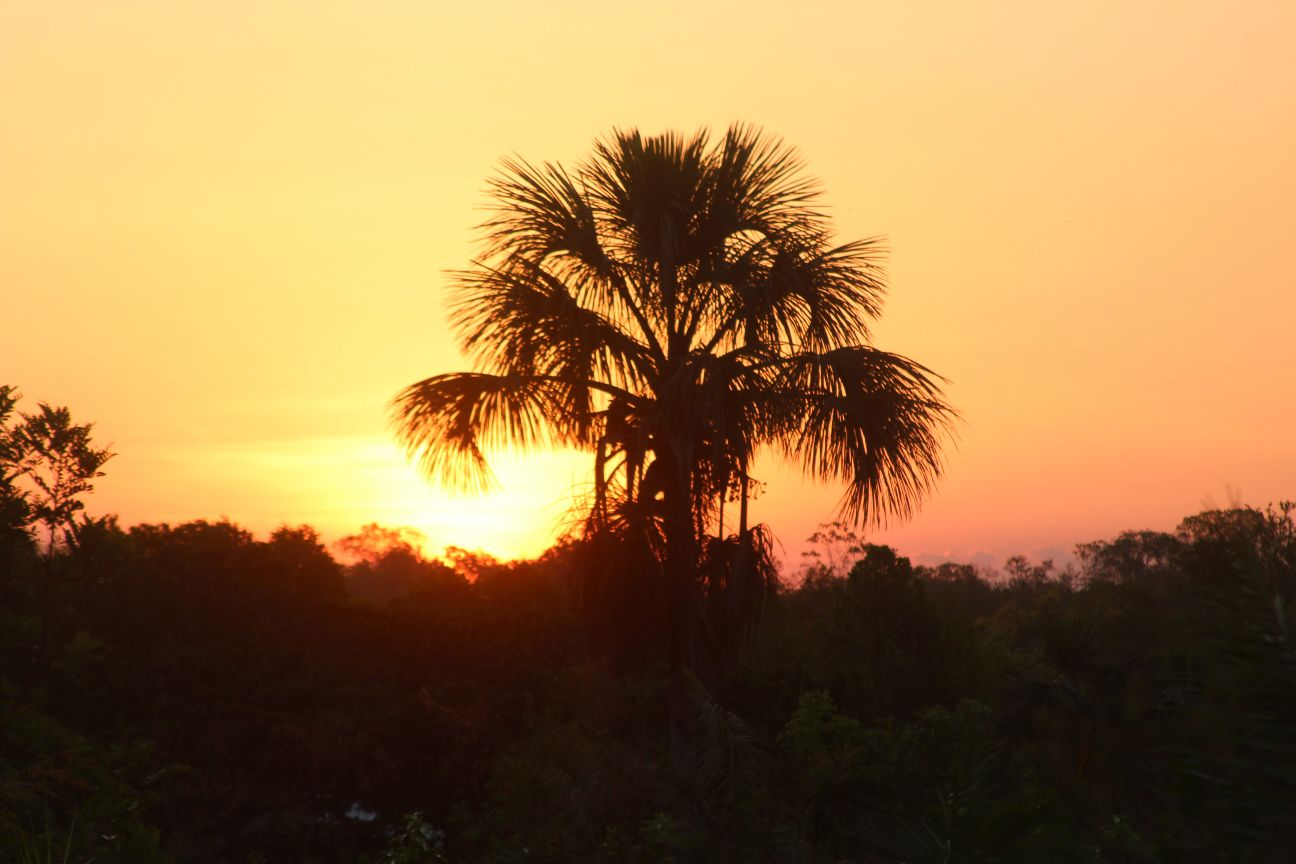
\includegraphics[scale=0.1]{Pordosol}
   \caption{Imagens lado a lado}\label{ladoalado}
\end{figure}
\end{lstlisting}
\end{tcolorbox}

\begin{figure}[H]
	\centering
	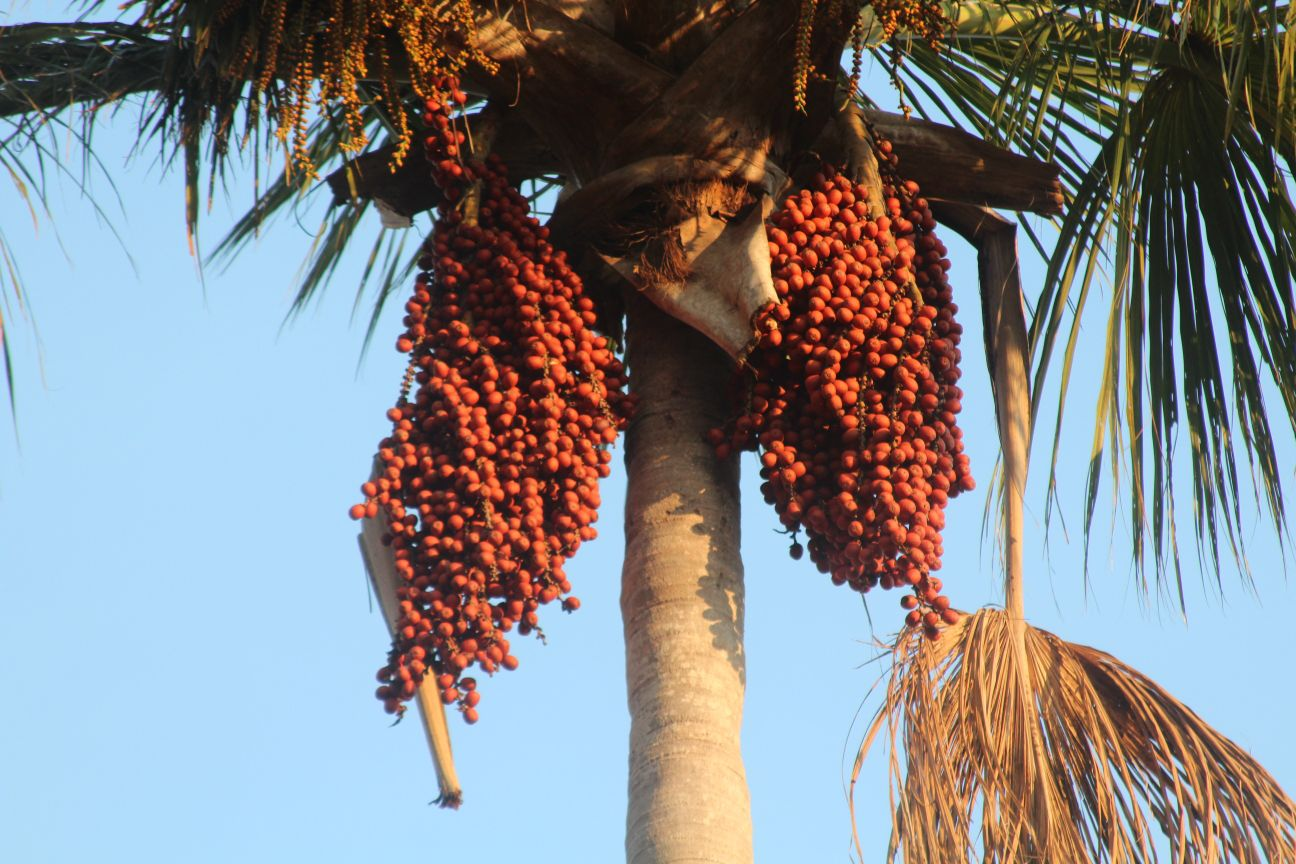
\includegraphics[scale=0.1]{Buriti}
	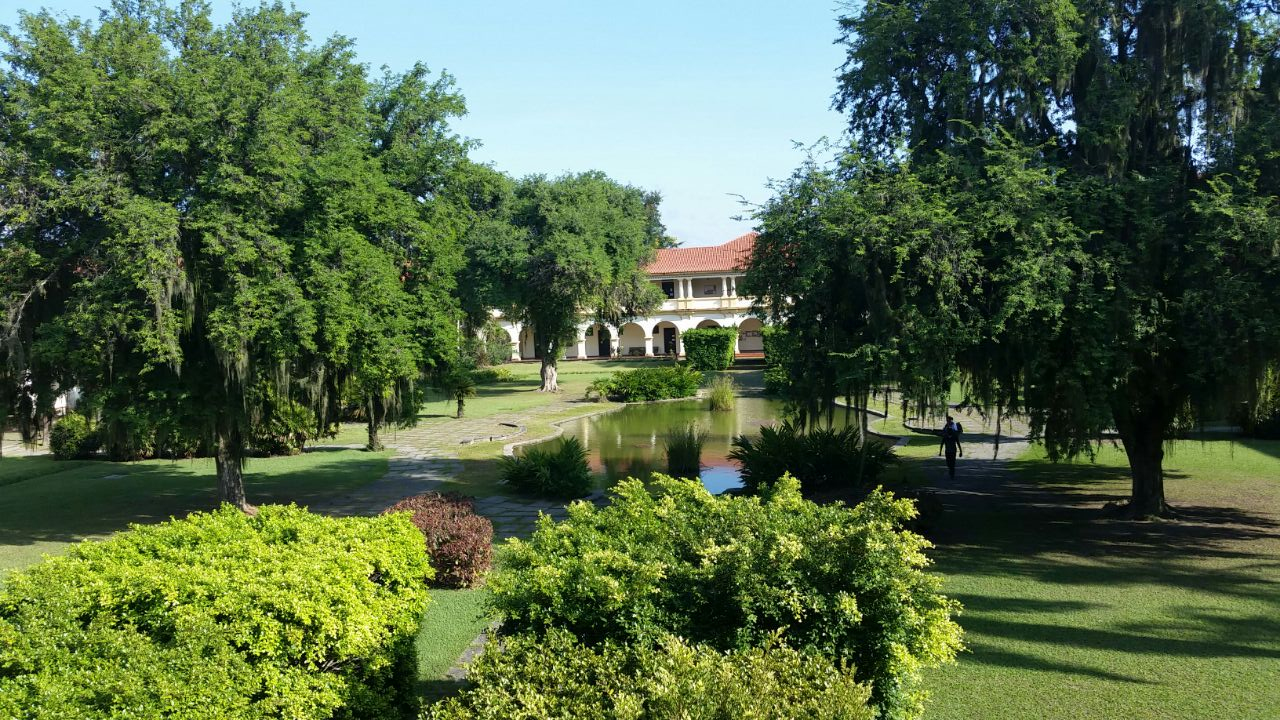
\includegraphics[scale=0.1]{RuralP1}
	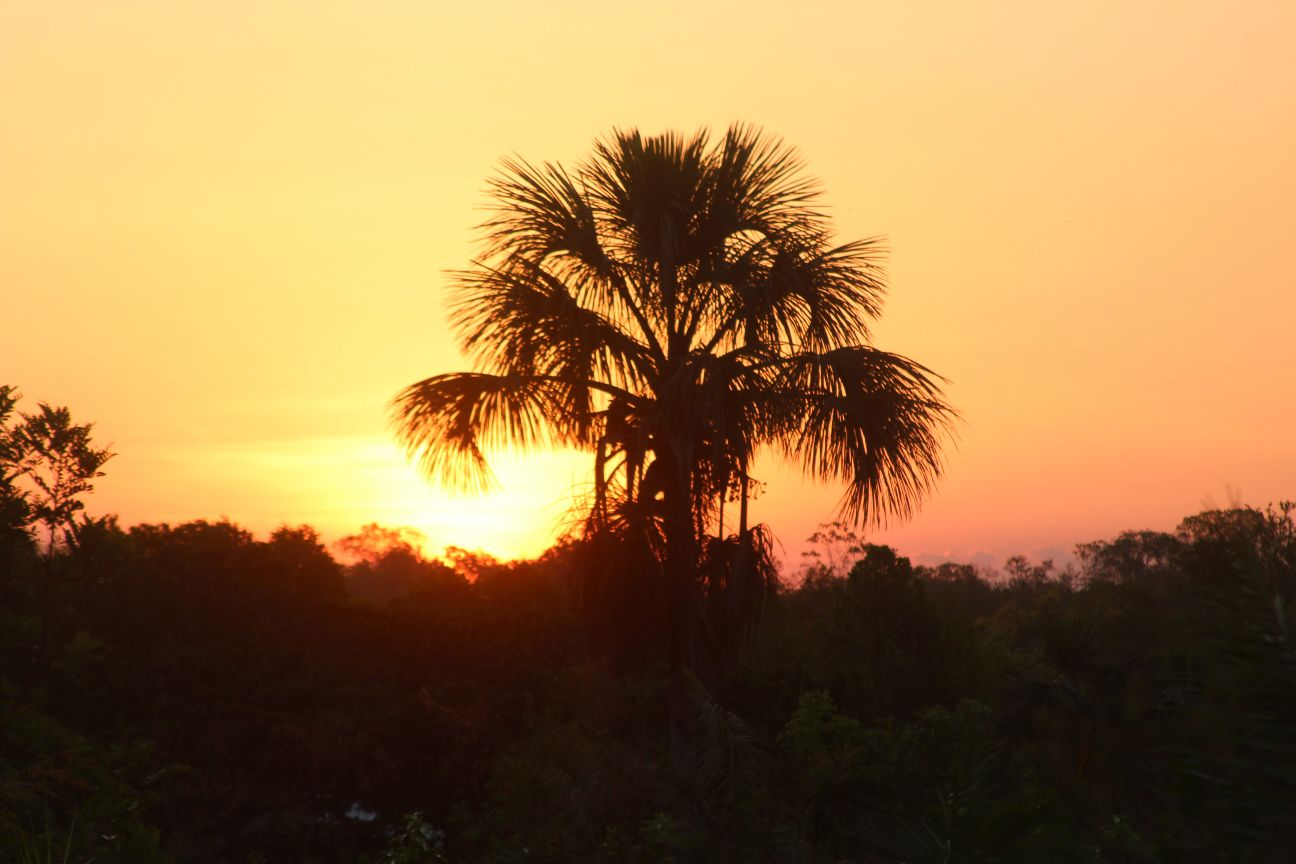
\includegraphics[scale=0.1]{Pordosol}
	\caption{Imagens lado a lado}\label{ladoalado}
\end{figure}

Para inserir uma legenda para cada figura e uma legenda geral tem-se a seguinte opção
\begin{tcolorbox}
\begin{lstlisting}
\begin{figure}[H]
   \centering
   \subcaptionbox{Fruta do buriti \label{fruta}}[0.33\linewidth]{%
		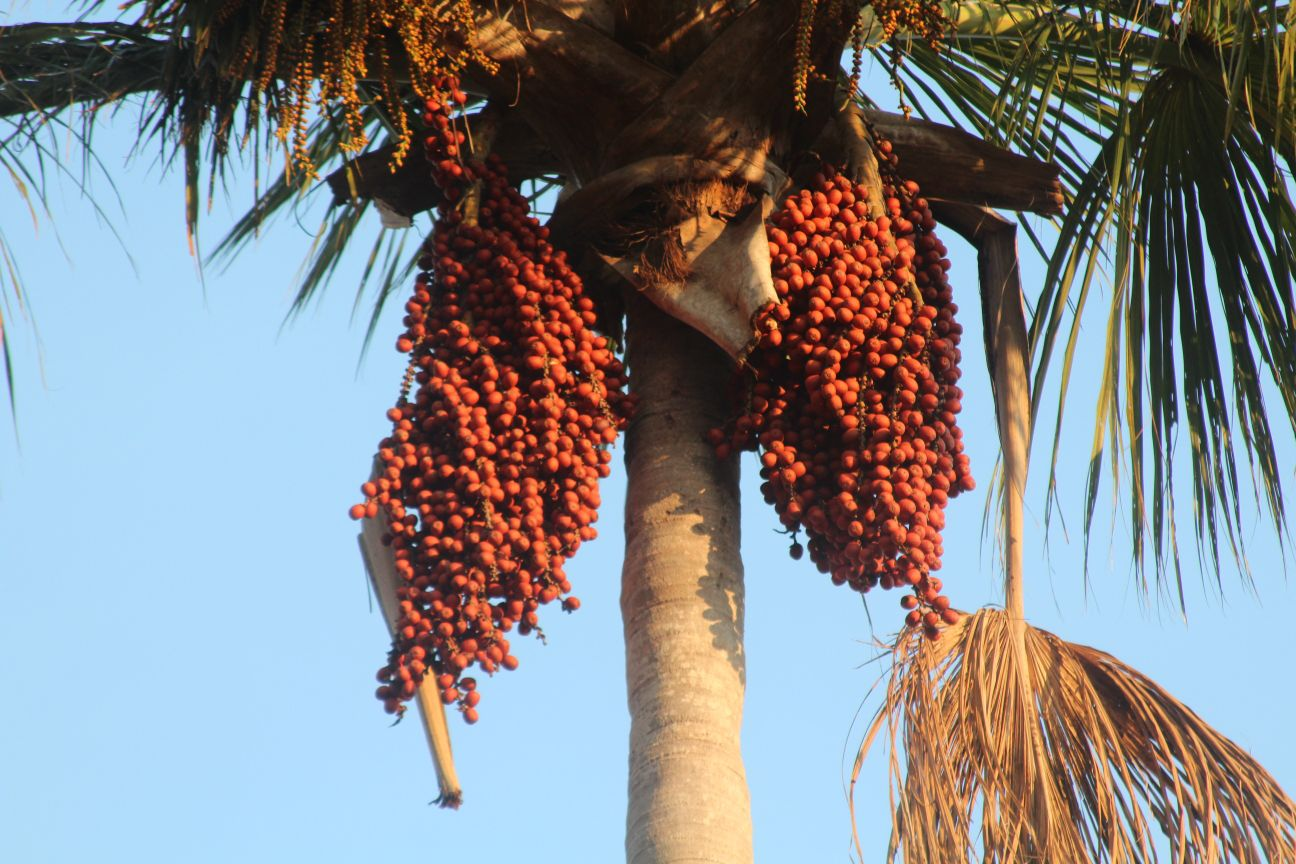
\includegraphics[scale=0.1]{Buriti}} %
   \subcaptionbox{Bonito por do sol e uma sublegenda intencionalmente
        grande\label{Pordosol}}[0.33\linewidth]{%%%
        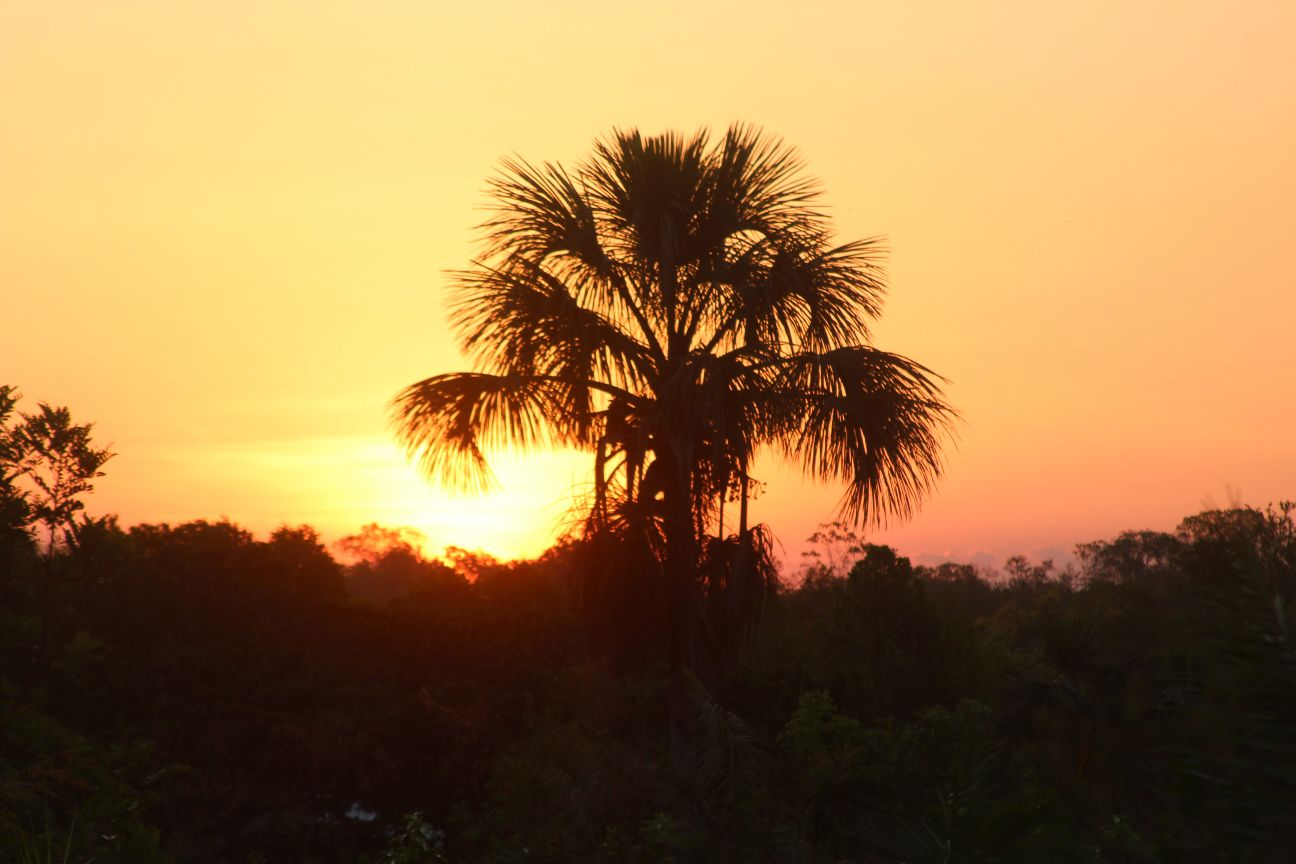
\includegraphics[scale=0.1]{Pordosol}}
   \subcaptionbox {Duas palmeiras de buriti \label{duas}}[%%%
        0.3\linewidth]{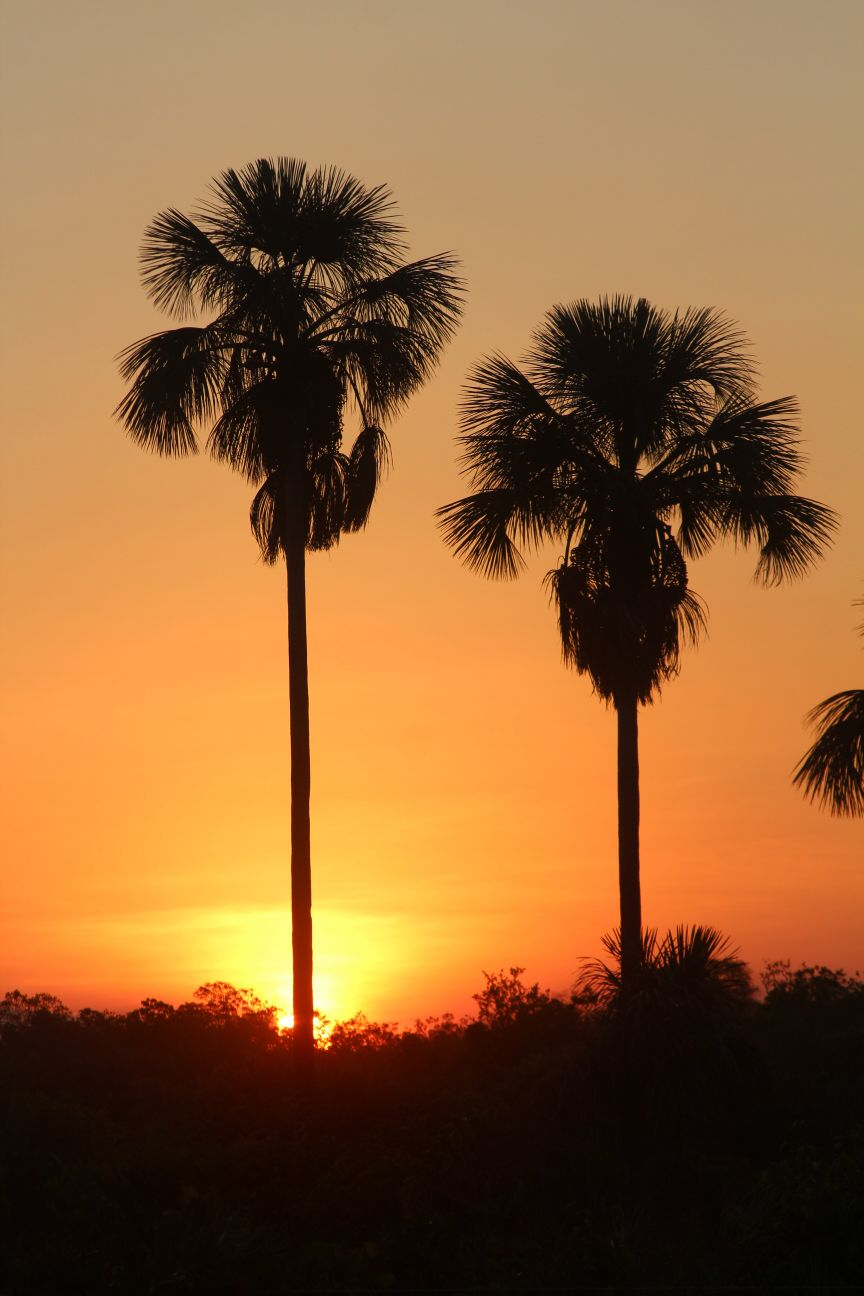
\includegraphics[scale=0.12]{Buritis}} %
   \caption{Buriti é uma palmeira de fruto saboroso}\label{buritis}
\end{figure}
\end{lstlisting}
\end{tcolorbox}

\begin{figure}[H]
	\centering
	\subcaptionbox{Fruta do buriti \label{fruta}}[0.33\linewidth]{%
		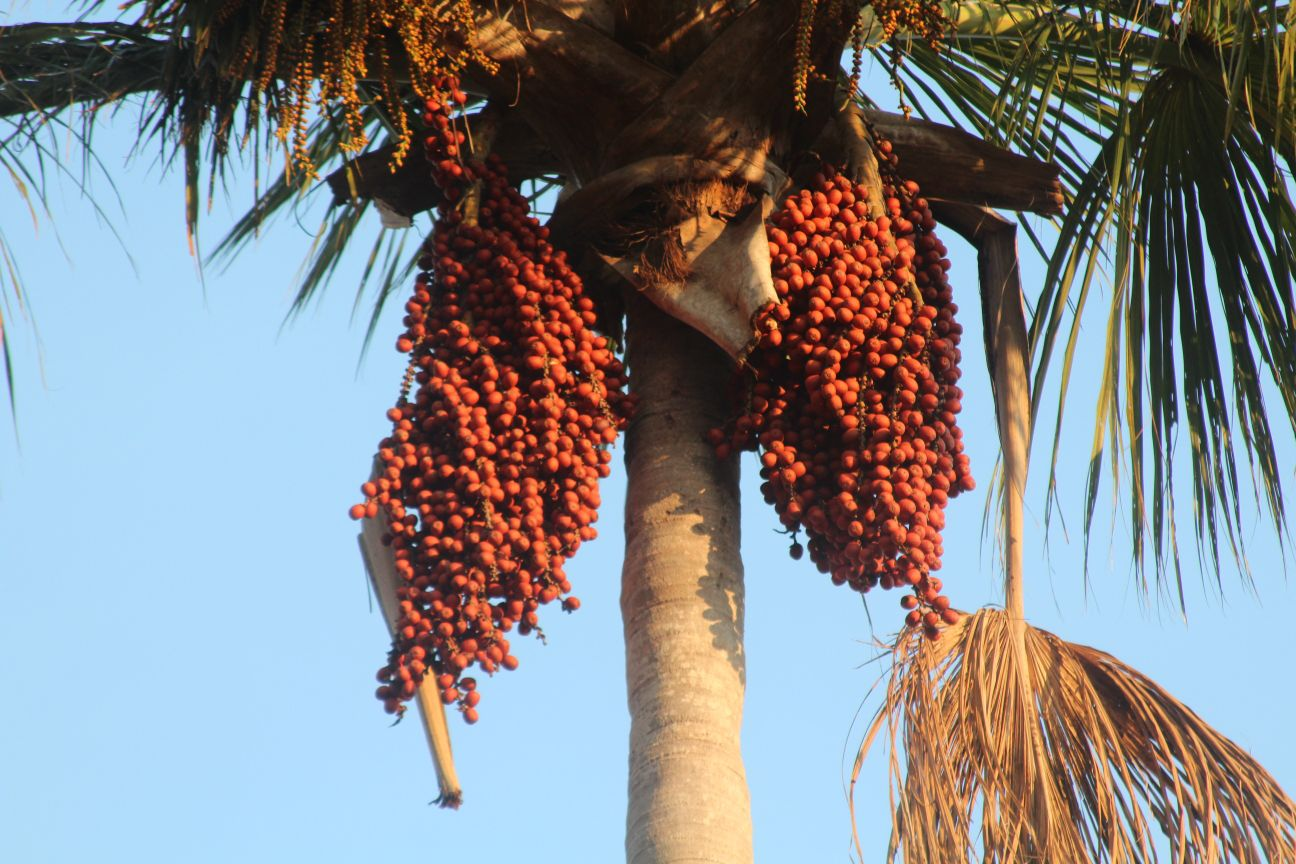
\includegraphics[scale=0.1]{Buriti}} %
	\subcaptionbox{Bonito por do sol e uma sublegenda intencionalmente grande
		\label{Pordosol}}[0.33\linewidth]{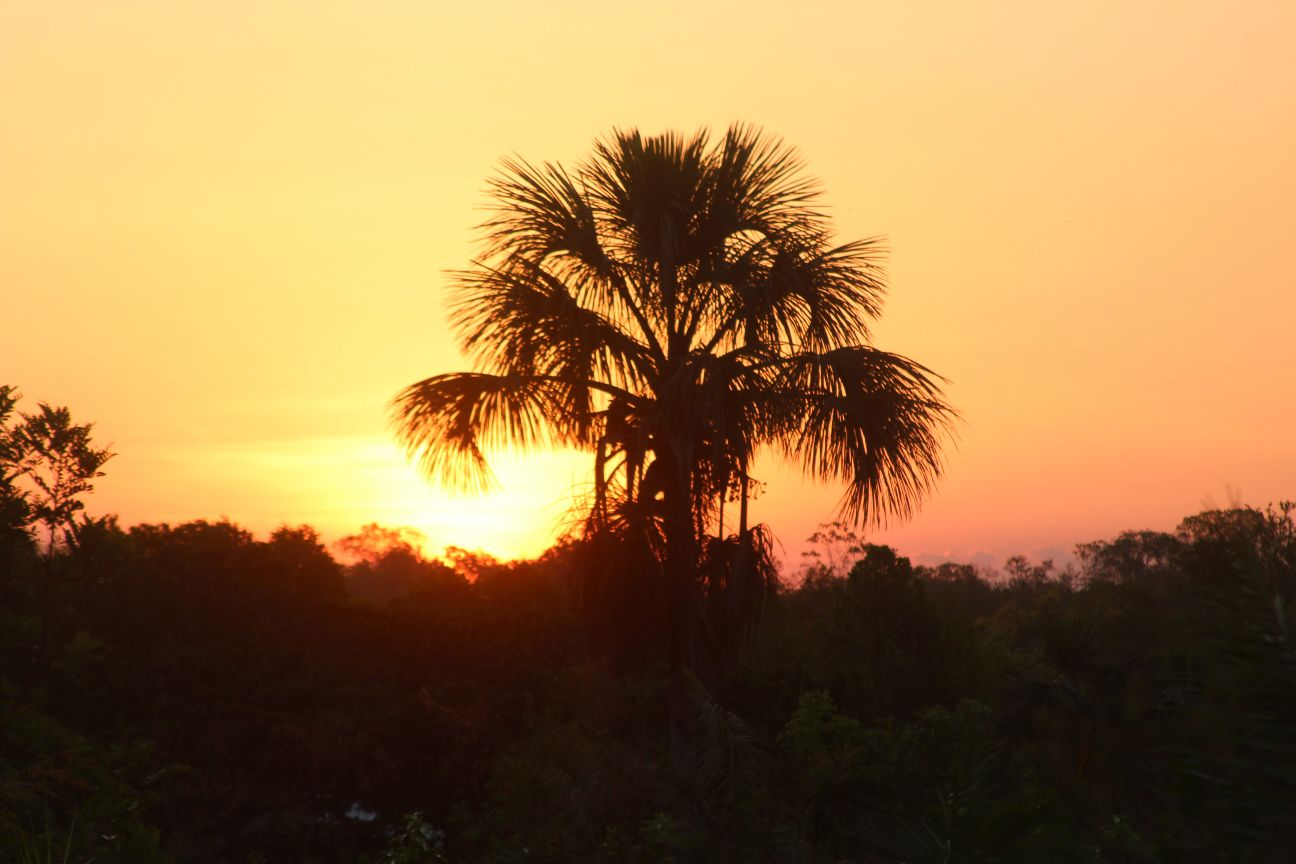
\includegraphics[scale=0.1]{Pordosol}}
	\subcaptionbox {Duas palmeiras de buriti \label{duas}}[0.3\linewidth]{%%%
		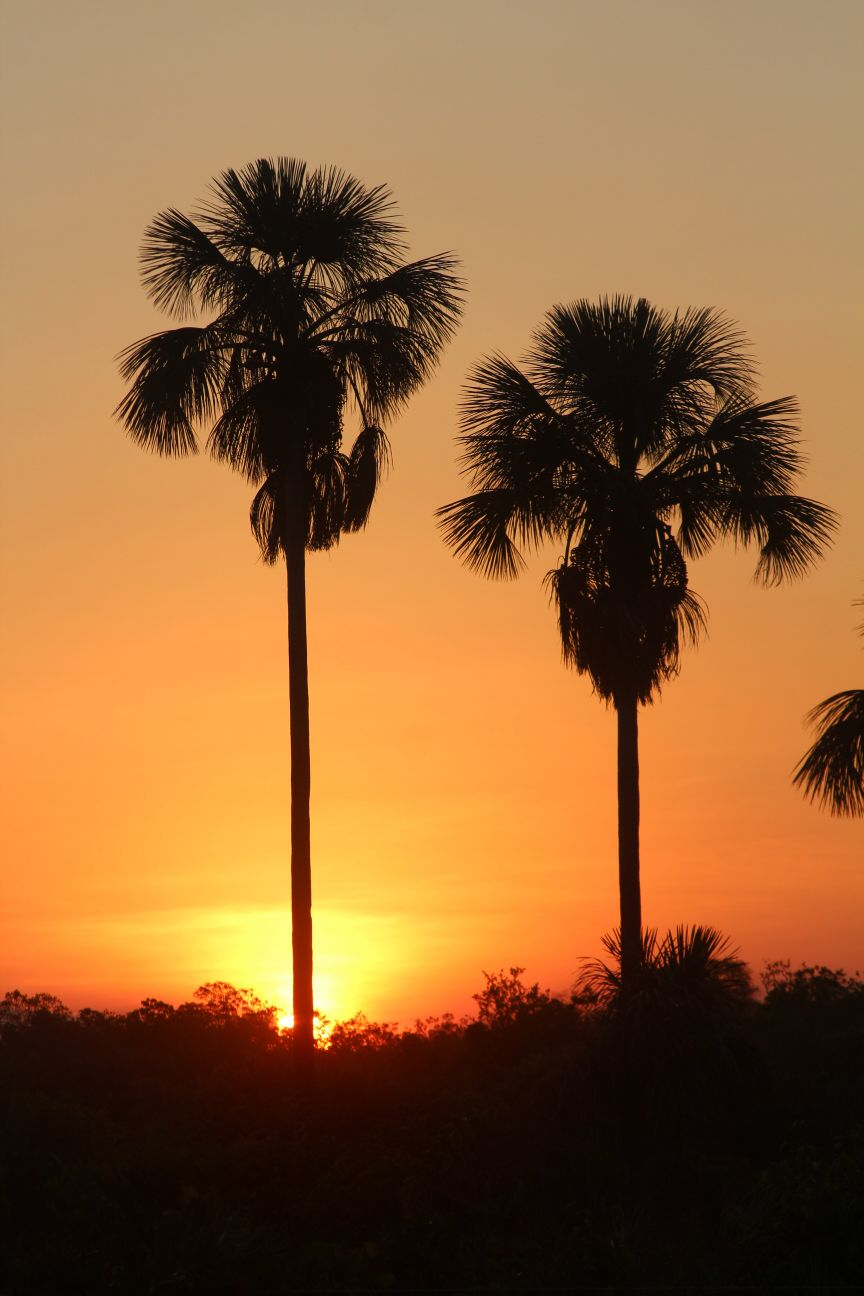
\includegraphics[scale=0.12]{Buritis}} %
	\caption{Buriti é uma palmeira de fruto saboroso}\label{buritis}
\end{figure}


\section{Inclusão de imagem com a classe estilo}

O \LaTeX\ utiliza o comando \cmc{includegraphics}{imagem}, que pertence ao pacote \paco{graphicx}, para inserir imagem. Alternativamente a classe estilo definiu os comandos: \com{imagem},
\com{imagemlp} e \com{imagemlp} que também exigem o pacote \paco{graphicx}. Esses comandos são muito parecidos, o primeiro insere a imagem em tamanho natural, o segundo ajusta a largura da imagem à largura da página sem provocar distorções, ambos possuem três argumentos, um opcional e dois obrigatórios. O \com{imagemlp}  ajusta a largura da imagem à largura da página sem criar distorções, não admite legenda e admite um argumento opcional. Sintaxe

\begin{center}
	\cmcc{imagem}{opções}{nome do arquivo}{legenda}
	
	\cmcc{imagemlp}{opções}{nome do arquivo}{legenda}
	
	\cmco{imagemsl}{opções}{nome do arquivo}
\end{center}
O parâmetro opções é opcional, ele aceita as mesmas chaves do 
parâmetro opcional do \com{includegraphics}. Nesses comandos o 
nome do arquivo é também a marca para fazer referência cruzada, 
assim o usuário é poupado de inventar apelidos para suas imagens 
e de inserir o comando \cmc{label}{marca} em cada uma de suas 
imagens para fazer referência cruzada.

Tanto o \coma{imagem} quanto o \coma{imagemlp} inserem a imagem 
dentro de um ambiente \ttt{table} carregado com o posicionador H, 
isso implica que a imagem ficará onde foi inserida de qualquer jeito.

A imagem~\ref{primeira} foi inserida com o código
\begin{tcolorbox}
\begin{lstlisting}
\begin{figure}[H]
   \centering
   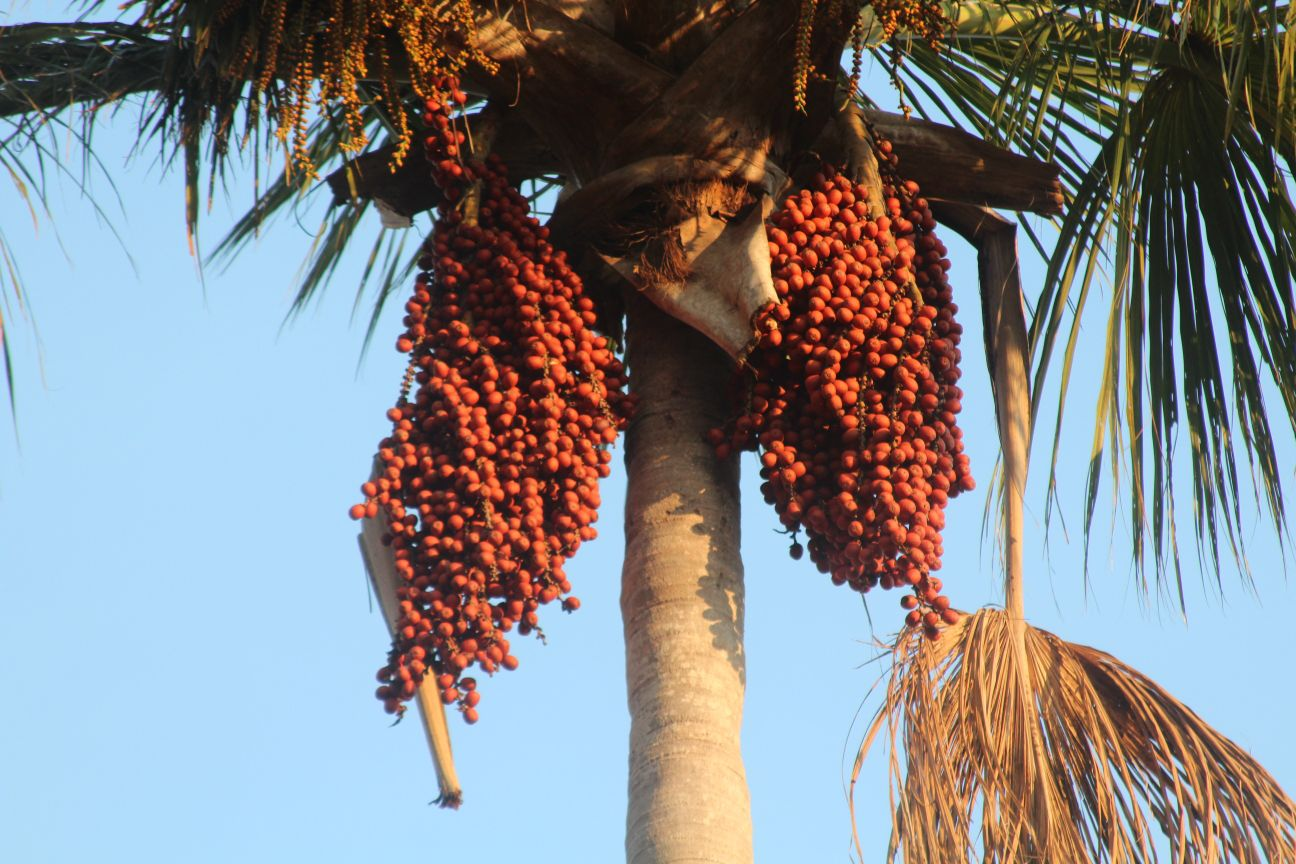
\includegraphics[scale=0.15]{Buriti}
   \caption{Imagem reduzia a $15\%$ do seu tamanho}
\end{figure}
\end{lstlisting}
\end{tcolorbox}

O mesmo resultado é obtido com o singelo fragmento
\begin{center}
\cmcc{imagem}{scale=0.15}{Buriti}{Imagem reduzia a $15\%$ do seu tamanho}
\end{center}
\imagem[scale=0.15]{Buriti}{Imagem reduzia a $15\%$ do seu tamanho}

Além do nome mais simples esses comandos são fáceis de manipular, eles 
se encarregam de inserir bons adereços que uma imagem em geral requer, 
tornando significativamente mais simples e prática a manipulação de imagem.

A imagem~\ref{op1} foi inserida com o código
\begin{tcolorbox}
\begin{lstlisting}
\begin{figure}[H]
   \resizebox{\textwidth}{!}{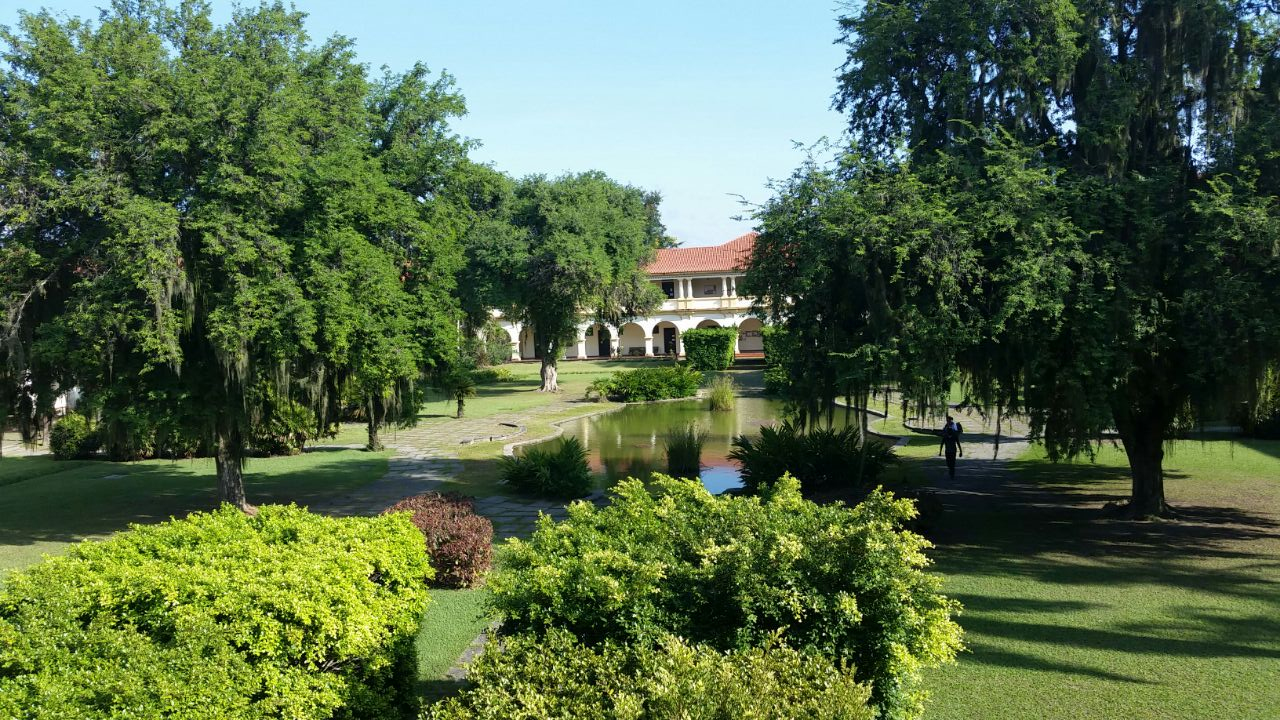
\includegraphics{RuralP1}}
   \caption{O prédio principal da UFRRJ, vulgo P1}
   \label{op1} %%% Marca para referência cruzada
\end{figure}
\end{lstlisting}
\end{tcolorbox}
O mesmo resultado é obtido com o código

\begin{center}
\cmc{imagemlp}{RuralP1}$\{$O prédio principal da UFRRJ, vulgo P1$\}$
\end{center}
\imagemlp{RuralP1}{O prédio principal da UFRRJ, vulgo P1}

\begin{tcolorbox}
\begin{lstlisting}
   Note que a imagem~\ref{RuralP1} foi ajustada para a largura da página, enquanto a imagem~\ref{Buriti}, por meio do argumento opcional $scale=0.15$, teve seu tamanho reduzido a $15\%$.
\end{lstlisting}
\tcblower
Note que a imagem~\ref{RuralP1} foi ajustada para a largura da página, enquanto a imagem~\ref{Buriti}, por meio do argumento opcional $scale=0.15$, teve seu tamanho reduzido a $15\%$.
\end{tcolorbox}

Observe como a referência cruzada foi feita utilizando o próprio nome do arquivo da imagem, sem necessidade de incluir o \cmc{label}{RuralP1} e \cmc{label}{Buriti}, essa é uma vantagem de usar os comandos \com{imagem} e \com{imagemlp} da classe estilo.

\begin{tcolorbox}
\begin{lstlisting}
\imagem[scale=0.8]{Esquema}{Imagem em pdf reduzida a $80\%$ de seu tamanho}
\end{lstlisting}
\end{tcolorbox}

\imagem[scale=0.8]{Esquema}{Imagem em pdf reduzida a $80\%$ de seu tamanho} 

\subsection*{Atenção!}
Os comandos \com{imagem} e \com{imagemlp} não podem ser utilizados para inserir a mesma imagem 
mais de uma vez no mesmo documento, se isso acontecer haverá duas imagens com a mesma marca no 
documento, essa inconsistência determina erro na construção de referência cruzada a essas imagens. 
Se for necessário inserir uma mesma imagem mais de uma vez no documento poderá ser utilizado um 
dos comandos \com{imagem} ou \com{imagemlp} para inserir a imagem uma vez e a outra deve ser 
incluída com o comando \com{includegraphics}, assim poderá ser utilizado o comando \cmc{label}{marca} 
para definir uma marca diferente para a segunda inclusão da imagem.